\documentclass[border=10pt]{standalone}
\usepackage{xcolor}
\usepackage{pgfplots}
\usepackage{tikz}
\begin{document}
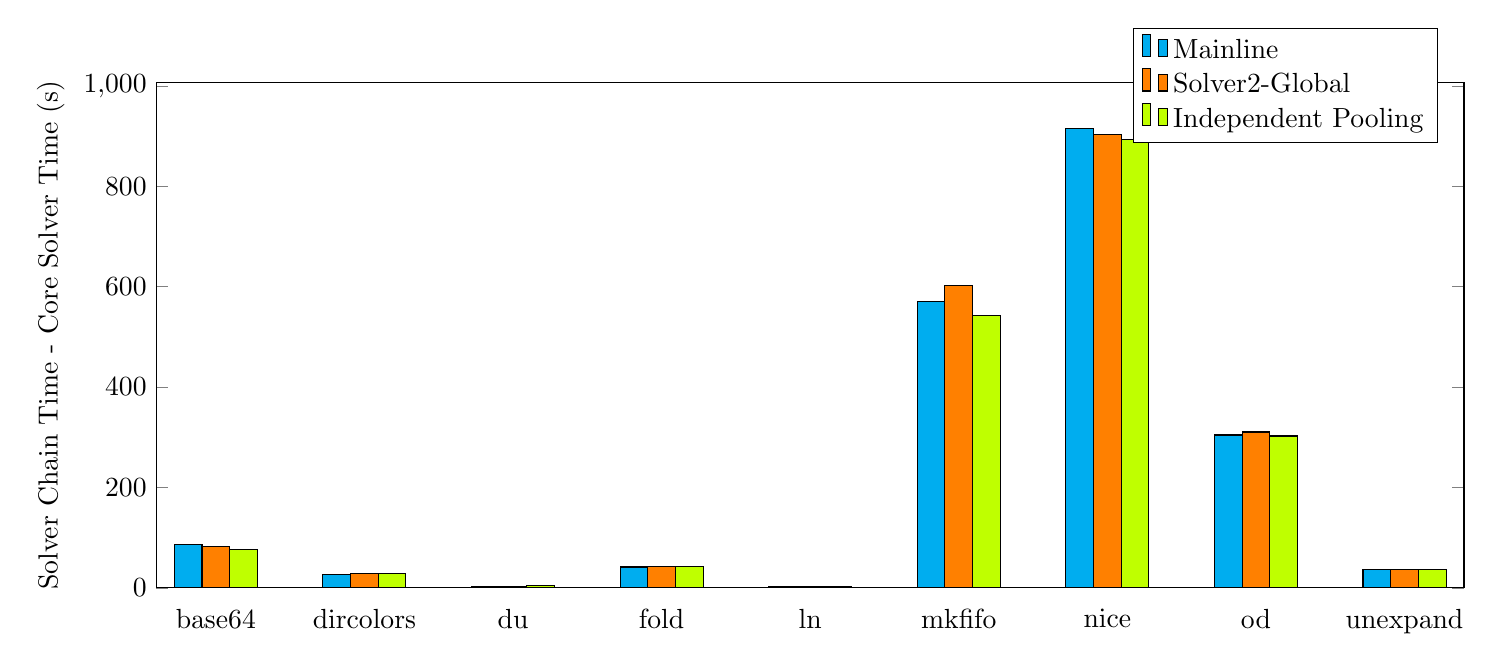
\begin{tikzpicture}
    \begin{axis}[
        width  = 1.5 * \textwidth,
        height = 8cm,
        major x tick style = transparent,
        % tickwidth=10,
        ybar=0,
        bar width=10pt,
        % ymajorgrids = true,
        ylabel = {Solver Chain Time - Core Solver Time (s)},
        symbolic x coords={base64,dircolors,du,fold,ln,mkfifo,nice,od,unexpand},
        xtick = data,
        scaled y ticks = false,
        enlarge x limits=0.05,
        ymin=0,
        legend cell align=left,
        legend style={
                at={(0.98,0.88)},
                anchor=south east,
                % column sep=1ex
        }
    ]
        \addplot[style={cyan,fill=cyan,mark=none}, draw=black]
	coordinates {(base64,85.97000000000025) (dircolors,27.56999999999971) (du,3.349999999999909) (fold,41.710000000000036) (ln,2.800000000000068) (mkfifo,569.97) (nice,915.02) (od,304.5) (unexpand,36.42999999999938)};
\addplot[style={orange,fill=orange,mark=none}, draw=black]
	coordinates {(base64,82.45000000000027) (dircolors,28.190000000000055) (du,3.3299999999999272) (fold,41.82999999999993) (ln,2.5300000000000296) (mkfifo,601.8399999999999) (nice,903.19) (od,310.46000000000004) (unexpand,36.25)};
\addplot[style={lime,fill=lime,mark=none}, draw=black]
	coordinates {(base64,76.92000000000007) (dircolors,28.769999999999982) (du,4.389999999999418) (fold,42.26999999999998) (ln,2.910000000000025) (mkfifo,541.8000000000001) (nice,893.0200000000001) (od,302.57000000000016) (unexpand,37.12999999999988)};

        \legend{Mainline,Solver2-Global,Independent Pooling}
    \end{axis}
\end{tikzpicture}
\end{document}
